% Stanford University PhD thesis style -- modifications to the report style
% This is unofficial so you should always double check against the
% Registrar's office rules
% See http://library.stanford.edu/research/bibliography-management/latex-and-bibtex
% 
% Example of use below
% See the suthesis-2e.sty file for documentation
%

% \documentclass[twoside,openright]{report}

\documentclass{report}
\usepackage{suthesis-2e}
\dept{Linguistics}
\submitdate{March 2024}

\usepackage[british]{babel}
\usepackage{lineno}
\usepackage{csquotes}

\usepackage[
backend=biber,
style=apa,
labeldate=year,
uniquename=false
]{biblatex}
\addbibresource{main.bib}

\usepackage[bookmarksnumbered=true,bookmarksopen=true,colorlinks=true,linkcolor=blue,citecolor=blue,filecolor=blue,urlcolor=blue]{hyperref}

\usepackage{fontspec}
\setmainfont{Times New Roman}

\usepackage{multicol,multirow}
\usepackage{float,graphicx}
\usepackage[table]{xcolor}
\usepackage{epigraph,ragged2e,booktabs,float,makecell,tocbibind,titlesec,capt-of,longtable,lipsum,pdflscape,silence}

\newcommand{\draft}[1]{{\color{red}#1}}
% Highlight post-defense corrections in blue for committee sign-off
% \newcommand{\corr}[1]{{\color{blue}#1}}

% Remove highlights for final version
\newcommand{\corr}[1]{#1}

\setcounter{tocdepth}{1}

\newcommand\blfootnote[1]{%
  \begingroup
  \renewcommand\thefootnote{}\footnote{#1}%
  \addtocounter{footnote}{-1}%
  \endgroup
}

% \chapternumberfont{\large} 
% \chaptertitlefont{\Large}

\titleformat{\chapter}[display]{\Large\bfseries}{\chaptertitlename\ \thechapter}{20pt}{\LARGE}

% \titleformat*{\section}{\fontsize{12}{15}\bfseries\selectfont}
% \titleformat*{\subsection}{\fontsize{10}{12}\bfseries\selectfont}

\usepackage{subfiles} % Best loaded last in the preamble

\begin{document}

% \linenumbers

\title{Improving access to untranscribed speech corpora using AI}
\author{Nay Myo San}
\principaladviser{Daniel Jurafsky}
\firstreader{Christopher Manning}
\secondreader{Arto Anttila}
 
\beforepreface

% Abstract must begin on page iv, 2 pages after the title page.
% (Stanford auto-inserts committee signature and copyright pages as ii and iii)
\prefacesection{Abstract}
\setcounter{page}{4}

How easily speech corpora can be indexed and searched has a direct impact on how effectively its contents can be used by many interested parties --- from linguists, to language teachers, to community members.~As transcribing speech is much more time consuming than recording it, large parts of speech corpora typically remain untranscribed, making it difficult to index and search these sub-parts.~While searchable transcriptions can be automatically derived using a speech-to-text system for major languages like English, such technologies are typically unavailable for smaller languages, especially those typical in language documentation work.~For documentation projects, this difficulty creates a bottleneck for creating language learning materials for language revitalisation and maintenance as well as linguistic analyses.~In this dissertation, I propose four approaches to widen this bottleneck to enable some form of search or indexing, or accelerate the time-consuming process of transcription.~Each chapter addresses a common but distinct scenario within language documentation projects according to the types and amounts of available data.~For each scenario, I propose a context-appropriate, data-efficient solution that leverages AI speech models as well as external resources where appropriate.

\prefacesection{Acknowledgments}

As stated in the title page, this dissertation is only a \emph{partial fulfilment} of the requirements --- certainly a major step but nonetheless one of many in a long journey.~I could not have completed this journey without the support of many within Stanford Linguistics and beyond who helped to make it a very fulfilling one.

First, I would like to thank those who not only made it possible for me to even start this journey but also be as prepared as possible for it.~I thank Kate Lindsey for paving the way through Stanford Linguistics, exemplifying (and advising me on) ways of combining and complementing the resources and expertise of the department with those beyond --- including a one-year deferral prior to starting the doctoral program.~I thank Jane Simpson and Nick Thieberger for finding the funds to support me for an extra year at CoEDL (ARC Centre of Excellence for the Dynamics of Language).

This time I spent at CoEDL both impacted the direction of my doctoral studies and enhanced the quality of it.~The first Transcription Acceleration Project workshop in June 2017 where I would first meet Daan van Esch and Ben Foley and others would sow the seeds for publications that would eventually form part of my dissertation.~Drawing on real-world linguistic fieldwork data for several of these publications would not have been possible without the connections with fieldwork linguists I made through my time at CoEDL.~Beyond work, I owe a massive thank you to Hedvig Skirg\r{a}rd, Stephen Mann, David Nash, Alex Marley, James Grama, Melody Ross, Sunny Ananthanarayan, Tina Gregor, Lauren Reed, Julia Miller, Mark Ellison, Bruno Olsson, Melea Vera and Cael Daniel who all made Canberra a truly joyful place --- from weekly Frinks (Friday drinks) at the University House, to board game nights playing Articulate, to music jam nights on stage at Smith's.

I'm grateful to Lily Clifford and Elisa Kreiss who made up our tiny cohort of three, sharing many of the excitements and stresses of first year including many early mornings (e.g.~attending lexical semantics classes) and late nights (e.g.~finishing lexical semantics homework).~I'm also grateful that the start of my Stanford journey overlapped with the final years of Kate Lindsey, Simon Todd, and Rob Voigt each of whom was able to impart much wisdom before their departures.~I thank Rob in particular for leading by example on how to gently but persuasively encourage participation in the department band.~I hope I have imparted as much to the now band (co-)leaders: Irene Yi, Yin Lin Tan and Antón de la Fuente.

There are two timely, cold e-mails that were pivotal to the direction of my dissertation.~First, I thank Steven Bird for e-mailing me a draft of his Sparse Transcription paper in May 2020.~This e-mail and subsequent discussion led to the experiments that became a qualifying paper.~Second, I thank Martijn Bartelds for replying to my cold e-mail enquiring about his recent arXiv paper in December 2020, when I was pondering follow up experiments.~This series of e-mail discussions then led to a published paper, then several more (four in total), his short visit to Stanford (Fall quarter 2022) and now a longer one as a post-doc.~I'm forever grateful to Martijn for the many brainstorming meetings, puzzling code debugging and intense last-minute writing marathons.

In the most literal sense, this dissertation would not have come together without the help of Dan Jurafsky.~I will never forget last two weeks of January 2024 in which I assembled four separate publications into a relatively coherent story that became this dissertation.~I am eternally grateful to Dan for being essentially on-call during this period, reading drafts of each chapter as I finished them, and helping triage the most important changes to be done given the time constraints (I also thank my committee Arto Anttila, Chris Manning as well as Karen Livescu and Laura Gwilliams for discussion and feedback at my defence that greatly improved the final dissertation).~Beyond this particular period, I am also grateful to Dan for his open, trusting, and patient approach to advising.~I was able to explore in my own time topics that interested me, come to him for advice when I was puzzled, and let projects and publications emerge out of my curiosity of finding ways to leverage these newly developed speech models for supporting language documentation work. 

I would like to thank the many people who have made the East Bay a wonderful home for me.~Prior to their move to Montreal, I thank Eva Portelance and Steven Rygaard hosting many dinner parties and impromptu backyard/porch hangouts.~I'm thankful to my book club buddies Ben McCutcheon and Allison Beer, and Andrew Westphal and Kim Taylor for the fortnightly Irish traditional music sessions at their house, and Geoff Bacon and Joshua Hurwitz for the East Bay cycling adventures.~I thank my former cohort mate, current housemate and future workmate Lily Clifford for many fun hangouts from guitar/fiddle jams to Berkeley Bowl and Viks runs --- cheers, mate!~Last but not least, I thank my partner Katie Coffey for her enthusiastic and unwavering support, cheering me on in the last stretch and helping proofread the entire dissertation.~I'm also grateful to the Coffey family (Kathy, Sean, Liz, Jay, Colleen, David, and Hilary) who have welcomed me into their lives, from the Thanksgiving/Christmas events to annual Watsonville/Tahoe trips as well as corgi updates and weekend tennis practice.~I look forward to spending more time again with all of you in the months ahead and beyond.

\afterpreface

\subfile{chp-intro}

\subfile{chp-speech-proc}

\subfile{chp-2021-asru}

\subfile{chp-2022-computel-5}

\subfile{chp-2023-computel-6}

\subfile{chp-2024-sigtyp}

\subfile{chp-conclusion}

\appendix
\chapter{Fine-tuning with a re-initialised final layer}
\label{sec:appendix}

In this section, we describe an earlier set of ASR fine-tuning experiments which were analogous to those reported in §\ref{sec:computel5-asr}, except for the manner in which vocabulary (i.e.~character set) was configured.~Following recommended fine-tuning practice,\footnote{\url{https://huggingface.co/blog/fine-tune-wav2vec2-english}} we initialised a linear layer whose output size corresponds to set of characters to be predicted (e.g. `A', `B', ...) and is derived from the target training dataset.~However, this guidance presupposes that the pre-trained model being fine-tuned is one with no prior fine-tuning for ASR on the same language.

Given the size of our available training data (total 65 minutes), we chose to continue to train the Robust wav2vec 2.0 model,\footnote{\url{https://huggingface.co/facebook/wav2vec2-large-robust-ft-swbd-300h}} already fine-tuned for English ASR on 300 hours of Switchboard \parencite{godfrey1992switchboard}.~The results of fine-tuning this model using various-sized subsets of our training data is reported below in Table \ref{tab:w2v2-datasets-old}.~Notably, fine-tuning with only 13 minutes of data resulted in a significantly worse than off-the-shelf performance (98\% vs. 37\%, off the shelf).~By deriving labels for the linear layer from our training dataset, the label mappings were scrambled (e.g. from Output 4 = `E' to Output 4 = `C'), yielding gibberish predictions during initial fine-tuning.~Through this fine-tuning process, 39 minutes of training data were required for the model to (re-)learn the appropriate parameters for English ASR.

\begin{table}[t]
% \vspace{1em}
\renewcommand{\arraystretch}{1.15}
\begin{center}
\begin{tabular}{|l|c|c|}
\hline

\textbf{Training set size} & \textbf{WER} & \textbf{CER} \\ \hline

\makecell[l]{
a. 65 minutes (100\%)} & 11\% & 5\% \\ 
b. 52 minutes (80\%)  & 13\% & 5\%\\
c. 39 minutes (60\%)  & 16\% & 6\% \\
d. 26 minutes (40\%)  & 37\% & 14\% \\ 
e. 13 minutes (20\%)  & 98\% & 78\% \\ 
\hline

f. \makecell[l]{Off-the-shelf (0\%)} & 37\% & 22\% \\ \hline

\end{tabular}
\end{center}
\vspace{-0.5em}
\caption[Results of ASR model adaptation using a randomly-initialised final layer]{Word error rates (WERs) achieved from fine-tuning the same wav2vec 2.0 model (large-robust-ft-swbd-300h) over 50 epochs using various subsets of data from 65 minutes of Australian English archival audio data.}
\label{tab:w2v2-datasets-old} 
% \vspace{-1em}
\end{table}

By contrast, in our experiments reported above in §\ref{sec:computel5-asr}, we adapted our datasets to match the vocabulary of the tokeniser included with the off-the-shelf model.~By doing so, we were able to achieve better than off-the-shelf ASR performance using only 39 seconds of training data.

Yet, unlike those experiments reported above, the addition of a language model to models fine-tuned with a re-initialised vocabulary yielded better performance.~As shown in Figure \ref{fig:asr-exp3-old}, the mean WER of the models fine-tuned with 39 minutes of data and without a language model was found to be 19.5\% (SD: 2.98\%; range: 15--23\%).~When a bigram language model was included, we found that the mean WER decreased to 14\% (SD: 2.30\%; range: 11--18\%).~These findings suggest that while the addition of a language model can be beneficial more experimentation is needed to inform best practices for calibrating and/or weighting the language model in near-zero shot learning scenarios.

\begin{figure}[H]
  \centering
%   \vspace{1em}
  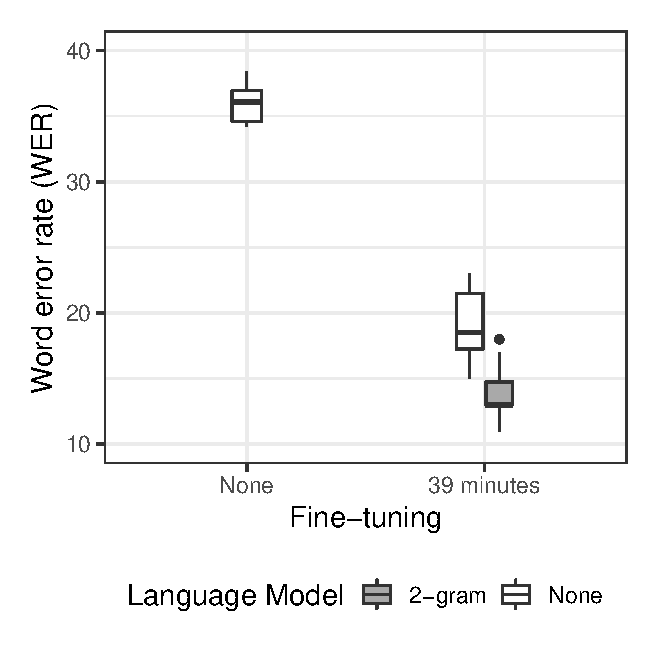
\includegraphics[width=0.45\linewidth]{figures/computel5-asr-reinit}
  \vspace{-1em}
  \caption[Results of adapting a ASR model by re-initialising the final layer and using various amounts of transcribed speech and with/without a language model]{Variability in word error rates of training and testing Robust wav2vec 2.0 models over 10 iterations using different samples in the training and testing datasets, holding constant the size of the training set (39 minutes) and testing set (16 minutes). The off-the-shelf model without fine-tuning was also evaluated on the same 10 testing sets.}
  \label{fig:asr-exp3-old}
  \vspace{-1em}
\end{figure}

\chapter{Continued pre-training and evaluation: materials and methods}
\label{sec:appendix-sigtyp2024}

\section{Data}

Galician, Spanish, Portuguese, and Indonesian data were sourced from CommonVoice \parencite{ardila2019common}; Setswana, Sesotho, and Sepedi from NCHLT \parencite{barnard2014nchlt}; Malay from MASS \parencite{tan2009mass}; and Iban from \textcite{juan2015using}.~For Iban only 7 hours of target data was available and for Sesotho/Sepedi only 56 hours per language of donor data was available.~Experiments were otherwise identical to the Indic experiments.

\section{Continued pre-training}

We carried out nearly identical experiments as the single-language experiments in \textcite{NOWAKOWSKI2023103148} for Ainu, as we obtained their configuration file for wav2vec 2.0 pre-training using the fairseq library.\footnote{\url{https://github.com/facebookresearch/fairseq}}~We made appropriate modifications to suit our hardware configuration (4 x A100 40GB GPUs), setting the batch size to 1.5M samples per GPU and gradient accumulation to 16 steps, yielding an effective batch size of 100 minutes.

As in other wav2vec 2.0 multilingual pre-training configurations~\parencite{conneau21_interspeech,babu22_interspeech,10.1609/aaai.v37i11.26521}, we form multi-lingual batches (specifically, \textit{bi-}lingual in our case).\footnote{Specifically, we use the implementation adapted from \url{https://github.com/AI4Bharat/IndicWav2Vec/}}~We set our sampling alpha to 0.0, which results in data being drawn uniformly from the two languages (i.e.~target is over-sampled).~We make this modification based on the CPT method in \textcite{paraskevopoulos2024sample}, where in- and out-of-domain Greek data were evenly sampled in each batch.~In this way, we consider this method akin to ``similar-language regularisation''~\parencite{neubig-hu-2018-rapid}, as we are more concerned with preventing over-fitting rather than learning about the donor data.

For each CPT run, we start from the official XLSR-128 model checkpoint and update the model for 10k steps.~We determined this value based on our pilot runs.~We found that 10k updates were sufficient to observe improved downstream ASR performance comparable to previous results \cite[e.g.][]{NOWAKOWSKI2023103148}.~This choice permitted us to maximise the number of languages compared in this paper, as each run required on average 15 hours (for 10k steps).
For select runs, we also verified that no further improvements could be obtained with additional updates (up to 20k).

\section{ASR fine-tuning and evaluation}

For ASR fine-tuning, we follow the official wav2vec 2.0 fine-tuning recipe suitable for 1 hour of transcriptions, modified for our hardware setup.~We use a single A6000 48 GB GPU with a batch size of 5.6M samples per GPU and accumulate gradients for 2 steps, yielding an effective batch size of 11.6 minutes.~As standard, the feature extractor is kept frozen across all updates and the transformer is frozen for the first 10k of 13k total updates, optimised using a CTC loss.~Each fine-tuning run required on average 3.5 hours.~For our findings to be applicable for languages with little external text data, we use Viterbi decoding without a language model to obtain transcriptions from the fine-tuned model for evaluation.

\section{ATDS analyses}

For all analyses, we trained the necessary \textit{k}-means and sentencepiece models on a random 5-hour subset of target language data (except for CommonVoice Punjabi, which had in total 4 hours available in the latest 15.0 release).~We adopted hyperparameters based on previous findings: extracting embeddings from the mid-point layer (12 of 24) of the XLSR-128 model \cite[e.g.][]{san2021leveraging,bartelds2022neural}, and \textit{k}=500 for \textit{k}-means and V=10k for the subword model which were reported as optimal values in \textcite{10096988}.~Using a 12GB 3060 GPU,~embedding extraction required about 10 minutes per data subset. The \textit{k}-means models trained in about 8 minutes and subword models in less than a minute.

For CommonVoice (CV) Punjabi and Hindi, we conducted similar analyses as those reported by \textcite[][Appendix D]{NEURIPS2020_92d1e1eb} for analysing correspondences between the wav2vec 2.0 code vectors and hand-aligned phone labels from TIMIT \parencite{Garofolo1993}.~In our case we used the labels for CV Punjabi and Hindi via grapheme-to-phoneme conversion, forced-aligned to the audio, and released as Praat TextGrids in the VoxCommunis corpus \parencite{ahn-chodroff-2022-voxcommunis}.~We then added tiers containing the wav2seq-induced labels.~We hand-inspected several TextGrids for data validation then compiled the correspondences between the wav2seq induced tokens and phoneme labels.~We make available all TextGrids as well as the aggregated data.

\clearpage
\addcontentsline{toc}{chapter}{Bibliography}
% Uncited entries included in the submitted (March 2024) bibliography
\nocite{chen2018almost,kahn2020self,menonFeatureExplorationAlmost2018,schneiderWav2vecUnsupervisedPretraining2019,tenney-etal-2019-bert}
\printbibliography

\end{document}